
%\documentclass{beamer}
\documentclass[handout]{beamer}
%\usepackage[latin1]{inputenc}
\usetheme{Warsaw}



\usepackage{amsmath}
\usepackage{amssymb}
\usepackage{amsthm}
\usepackage{amsfonts}
\usepackage{graphicx}
\usepackage{mathtools}
\usepackage{hyperref}

%\usepackage[g]{esvect}

\DeclarePairedDelimiter{\abs}{\lvert}{\rvert}
\DeclarePairedDelimiter{\ceil}{\lceil}{\rceil}
\DeclarePairedDelimiter{\floor}{\lfloor}{\rfloor}
\DeclarePairedDelimiter{\avect}{\langle}{\rangle}
\DeclarePairedDelimiter{\aset}{\allowbreak\lbrace}{\rbrace}

%\newcommand{\true}{\mathit{true}}
%\newcommand{\fals}{\mathit{false}}
\newcommand{\true}{\mbox{T}}
\newcommand{\fals}{\mbox{F}}
\newcommand{\Nat}{\mathbb{N}}
\newcommand{\Int}{\mathbb{Z}}
\newcommand{\defeq}{:=}
\newcommand{\transpose}{^ \top }
\newcommand{\queseq}{\overset{?}{=}}
%\newcommand{\transpose}{^ \intercal }
\newcommand{\pipe}{\,|\,}
\newcommand{\vbl}[1]{\ensuremath{\mathit{#1}}}
\newcommand{\detop}[1]{\det(#1)}
%\newcommand{\vect}[1]{\boldsymbol{\vbl{#1}}}
\newcommand{\vect}[1]{{\overrightarrow{#1}}}
\newcommand{\slfrac}[2]{\left.#1\middle/#2\right.}
%\newcommand{\vect}[1]{{\vv{#1}}}
\newcommand{\modop}[1]{\mbox{ mod }#1}
\newcommand{\mathsc}[1]{\text{\normalfont\scshape#1}}

\newcounter{exercisecnt}
\def\theexercisecnt{\arabic{exercisecnt}}
\newenvironment{exercise}
{\refstepcounter{exercisecnt}
 {\bf Exercise \theexercisecnt.}}
{}

\newcounter{exercisepartcnt}[exercisecnt]
\def\theexercisepartcnt{\theexercisecnt.\alph{exercisepartcnt}}
\newenvironment{exercisepart}
{\refstepcounter{exercisepartcnt}
 {\bf Exercise \theexercisepartcnt.}}
{}



%\usepackage{algorithm}
%\usepackage{algorithmicx}
%\usepackage{algorithm}% http://ctan.org/pkg/algorithms
%\usepackage{algpseudocode}% http://ctan.org/pkg/algorithmicx

\usepackage{tikz}
\usetikzlibrary{arrows}

\setbeamertemplate{navigation symbols}{}
\setbeamertemplate{bibliography item}[text]
\title{Search for Self-Stabilizing Protocols}
\author{Brandon Crowley \and Alex Klinkhamer \and Man Wang}
\institute{Michigan Technological University}
\date{2012}

\begin{document}

\setlength{\abovedisplayskip}{0.5em}
\setlength{\abovedisplayshortskip}{0.5em}
\setlength{\belowdisplayskip}{0.5em}
\setlength{\belowdisplayshortskip}{0.5em}
\setlength{\abovecaptionskip}{0.0em}
\setlength{\belowcaptionskip}{0.0em}

\begin{frame}
\titlepage
\end{frame}

\begin{frame}
\frametitle{Self-Stabilization}
\begin{itemize}
\item The $\vbl{invariant}$ is the set of states in which the system is expected to operate.
\item The protocol is considered to be converging if it can eventually transition to an invariant state
 \begin{itemize}
 \item A protocol is $\vbl{weakly}$ $\vbl{converging}$ if and only if, from every state outside the
    invariant, the invariant can be reached\cite{wssGouda01}.
 \item A protocol is $\vbl{strongly}$ $\vbl{converging}$ if and only if, from every state outside the
    invariant, the invariant must be reached.  This implies the protocol is livelock and deadlock
    free\cite{wssGouda01}.
 \end{itemize}
\item The goal of Self-Stabilization is to find an algorithm that can reach a legitimate state from
    any illegitimate state on its own.
\end{itemize}
\end{frame}

\begin{frame}
\frametitle{Sum-Not-2 Problem}
\begin{figure}
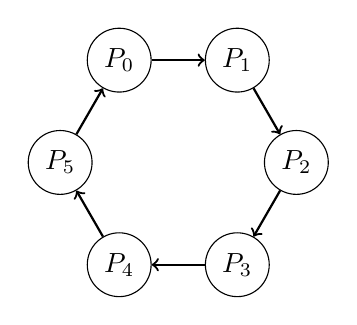
\begin{tikzpicture}[x=1.5cm,y=1.5cm]
\tikzstyle{every node}=[draw,circle]
\draw
 (0,0)      node (0) {$P_0$}
 ++(   0:1) node (1) {$P_1$}
 ++( -60:1) node (2) {$P_2$}
 ++(-120:1) node (3) {$P_3$}
 ++(-180:1) node (4) {$P_4$}
 ++(-240:1) node (5) {$P_5$}
 ;
\path[->,draw,thick]
(0) edge (1)
(1) edge (2)
(2) edge (3)
(3) edge (4)
(4) edge (5)
(5) edge (0)
;
\end{tikzpicture}

\begin{flushleft}
For all $i\in\Nat_6$,
\begin{eqnarray*}
P_i & : &
 \mbox{
  $\begin{cases}
  x_i\in\Nat_2 & \mbox{(read-write)} \\
  x_{i-1}\in\Nat_2 & \mbox{(read-only)} \\
  \end{cases}$
 }
\end{eqnarray*}
Invariant:
\[ I \equiv (\forall i\in\Nat_6: x_i + x_{i-1} \ne 2) \]
\end{flushleft}
\end{figure}
\end{frame}

\begin{frame}
\frametitle{Stabilizing Sum-Not-2 Transition Graph}
Stabilizing protocol for each process $P_i$:
\begin{eqnarray*}
   (x_i = 0) \wedge (x_{i-1} = 2) & \to & x_i \defeq 1;
\\ (x_i = 1) \wedge (x_{i-1} = 1) & \to & x_i \defeq 0;
\\ (x_i = 2) \wedge (x_{i-1} = 0) & \to & x_i \defeq 0;
\end{eqnarray*}
\begin{figure}
\centering
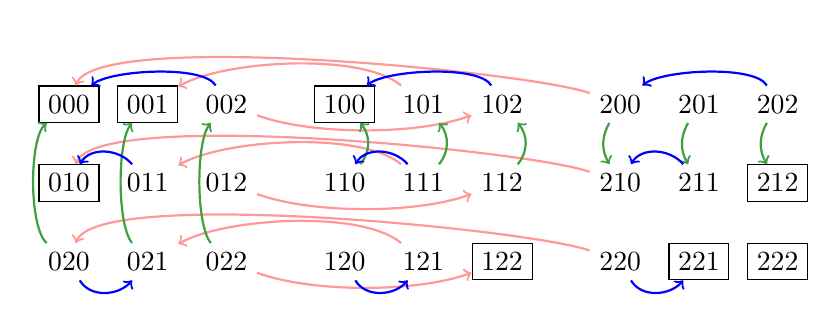
\begin{tikzpicture}[x=1.0cm,y=1.0cm]
\tikzstyle{every node}=[]
\tikzstyle{legit}=[draw]
\def \dx {3.5}
\draw
  (  0, 0) node [legit] (000) {000}
++(\dx, 0) node [legit] (100) {100}
++(\dx, 0) node         (200) {200}
  (  0,-1) node [legit] (010) {010}
++(\dx, 0) node         (110) {110}
++(\dx, 0) node         (210) {210}
  (  0,-2) node         (020) {020}
++(\dx, 0) node         (120) {120}
++(\dx, 0) node         (220) {220}
  (  1, 0) node [legit] (001) {001}
++(\dx, 0) node         (101) {101}
++(\dx, 0) node         (201) {201}
  (  1,-1) node         (011) {011}
++(\dx, 0) node         (111) {111}
++(\dx, 0) node         (211) {211}
  (  1,-2) node         (021) {021}
++(\dx, 0) node         (121) {121}
++(\dx, 0) node [legit] (221) {221}
  (  2, 0) node         (002) {002}
++(\dx, 0) node         (102) {102}
++(\dx, 0) node         (202) {202}
  (  2,-1) node         (012) {012}
++(\dx, 0) node         (112) {112}
++(\dx, 0) node [legit] (212) {212}
  (  2,-2) node         (022) {022}
++(\dx, 0) node [legit] (122) {122}
++(\dx, 0) node [legit] (222) {222}
;
\path[->,draw,thick]
(002) edge [color=red!40,out=- 20,in= 200,looseness=.7] (102)
(012) edge [color=red!40,out=- 20,in= 200,looseness=.7] (112)
(022) edge [color=red!40,out=- 20,in= 200,looseness=.7] (122)
(101) edge [color=red!40,out= 140,in=  30,looseness=.6] (001)
(111) edge [color=red!40,out= 140,in=  30,looseness=.6] (011)
(121) edge [color=red!40,out= 140,in=  30,looseness=.6] (021)
(200) edge [color=red!40,out= 160,in=  70,looseness=.3] (000)
(210) edge [color=red!40,out= 160,in=  70,looseness=.3] (010)
(220) edge [color=red!40,out= 160,in=  70,looseness=.3] (020)

(200) edge [color=green!50!black!75,out=-120,in= 120] (210)
(201) edge [color=green!50!black!75,out=-120,in= 120] (211)
(202) edge [color=green!50!black!75,out=-120,in= 120] (212)
(110) edge [color=green!50!black!75,out=  50,in=- 50] (100)
(111) edge [color=green!50!black!75,out=  50,in=- 50] (101)
(112) edge [color=green!50!black!75,out=  50,in=- 50] (102)
(020) edge [color=green!50!black!75,out= 140,in=-140,looseness=.5] (000)
(021) edge [color=green!50!black!75,out= 130,in=-130,looseness=.5] (001)
(022) edge [color=green!50!black!75,out= 130,in=-130,looseness=.5] (002)

(002) edge [color=blue,out= 120,in=  40,looseness=.5] (000)
(102) edge [color=blue,out= 120,in=  40,looseness=.5] (100)
(202) edge [color=blue,out= 120,in=  40,looseness=.5] (200)
(011) edge [color=blue,out= 130,in=  60] (010)
(111) edge [color=blue,out= 130,in=  60] (110)
(211) edge [color=blue,out= 130,in=  60] (210)
(020) edge [color=blue,out=- 60,in= 230] (021)
(120) edge [color=blue,out=- 60,in= 230] (121)
(220) edge [color=blue,out=- 60,in= 230] (221)
;
\end{tikzpicture}
\caption{Transitions of {\color{red!40} $P_0$}, {\color{green!50!black!75} $P_1$}, {\color{blue} $P_2$}. Legitimate states $x_0x_1x_2$ are boxed.}
\end{figure}
\end{frame}

\begin{frame}
\frametitle{Representing State Sets}
\begin{itemize}
\item A state is a valuation of variables.
 \begin{itemize}
 \item In PDDL, these are predicates and functions on objects.
 \end{itemize}
\item Can represent a set of states with a predicate formula.
 \begin{itemize}
 \item Ex: $x=1\vee y=0$ represents $3$ states of $2$ bits $x$ and $y$.
 \item Equivalently: $(x=0\wedge y=0) \vee (x=1\wedge y=0) \vee (x=1\wedge y=1)$.
 \end{itemize}
\item A predicate formula can be represented by...
 \begin{itemize}
 \item Binary decision diagram (BDD) if all variables are Boolean.
 \item Multi-valued decision diagram (MDD) if all variables are finite.
 \end{itemize}
\end{itemize}
\end{frame}

\begin{frame}
\frametitle{Representing Transition Sets (Actions)}
\begin{itemize}
\item Introduce primed variables for destination variables.
\item Example:
 \begin{itemize}
 \item Consider an action $A$.
  \begin{itemize}
  \item[] Precondition: $y < 20$.
  \item[] Effect: $x \defeq x - y$.
  \end{itemize}
 \item As a formula: $A = (y < 20) \wedge (x' = x - y) \wedge (y' = y)$
 \end{itemize}
\end{itemize}
\end{frame}

\begin{frame}
\frametitle{Representing State Sets by MDD}
In the $3$ process example of Sum-Not-2, the actions of $P_1$ could be represented by the following formula:
\[\begin{array}{rl}
   ( & ((x_1 = 0) \wedge (x_0 = 2) \wedge (x_1' = 1))
\\ \vee & ((x_1 = 1) \wedge (x_0 = 1) \wedge (x_1' = 0))
\\ \vee & ((x_1 = 2) \wedge (x_0 = 0) \wedge (x_1' = 0))
\\ ) &
\\ \wedge & (x_0 = x_0')
\\ \wedge & (x_2 = x_2')
\end{array}\]
\end{frame}

\begin{frame}
\frametitle{Image}
\begin{itemize}
\item The $\vbl{image}$ function finds all states which transitions $T$ map from $S$.
 \begin{itemize}
 \item $\vbl{image}(T,S) = \aset{s_1 \in \mathcal{S} \pipe\exists s_0\in S : (s_0,s_1)\in T}$
 \end{itemize}
\item Compute using standard operations.
 \begin{itemize}
 \item Conjunct the formulas of $S$ and $T$.
 \item Project out unprimed variables with existential quantification.
 \item Change primed variables to unprimed.
 \end{itemize}
\item Example:
 \begin{itemize}
 \item Let action $A = (y < 20) \wedge (x' = x - y) \wedge (y' = y)$.
 \item $\vbl{image}(A, (y > 3) \wedge (x = 2))$
 \\$= \vbl{unprime}(\exists x,y : (y > 3)\wedge (x = 2) \wedge A)$
 \\$= \vbl{unprime}((y' > 3) \wedge (y' < 20) \wedge (x' = 2 - y'))$
 \\$= (y > 3) \wedge (y < 20) \wedge (x = 2 - y)$
 \end{itemize}
\end{itemize}
\end{frame}

\begin{frame}
\frametitle{Preimage}
\begin{itemize}
\item The $\vbl{preimage}$ function finds all states which are mapped to states in $S$ by transitions $T$.
 \begin{itemize}
 \item $\vbl{preimage}(T,S) = \aset{s_0 \in \mathcal{S} \pipe\exists s_1\in S : (s_0,s_1)\in T}$
 \end{itemize}
\item Compute using standard operations.
 \begin{itemize}
 \item Prime all variables in formula of $S$.
 \item Conjunct with formula of $T$.
 \item Project out primed variables with existential quantification.
 \end{itemize}
\item Example:
 \begin{itemize}
 \item Let action $A = (y < 20) \wedge (x' = x - y) \wedge (y' = y)$.
 \item $\vbl{preimage}(A, (y > 3) \wedge (x = 2))$
 \\$= \exists x',y' : \vbl{prime}((y > 3)\wedge (x = 2)) \wedge A$
 \\$= \exists x',y' : (y' > 3)\wedge (x' = 2) \wedge A$
 \\$= (y > 3) \wedge (y < 20) \wedge (x = y + 2)$
 \end{itemize}
\end{itemize}
\end{frame}

\begin{frame}
\frametitle{Search Algorithm Initialization}
\begin{enumerate}
\item Let $\vbl{candidates}$ be a list of all actions.
\item Prune all actions which are self-loops from $\vbl{candidates}$.
 \begin{enumerate}
 \item[] Example self-loop: $x_1 = 1 \wedge x_0 = 0 \to x_1\defeq 1$.
 \end{enumerate}
\item Prune all actions which break closure from $\vbl{candidates}$.
\item Let $\vbl{actions}$ be an empty list actions.
\item Call backtracking algorithm.
\end{enumerate}
\end{frame}

\begin{frame}
\frametitle{Backtracking Algorithm}
\begin{enumerate}
\item If all deadlocks in illegitimate states are resolved by $\vbl{actions}$, return success!
\item While $\vbl{actions}\cup\vbl{candidates}$ weakly converge to the invariant,
 \begin{enumerate}
 \item Pick an action $B\in\vbl{candidates}$ using most-constrained deadlock heuristic.
 \item Let $\vbl{actions'} \defeq \vbl{actions} \cup \aset{B}$.
 \item Let $\vbl{candidates'} \defeq \vbl{candidates} \setminus \aset{B}$.
 \item Perform forward checking on $\vbl{actions'}$ and $\vbl{candidates'}$ to shrink $\vbl{candidates'}$.
 \item {\bf Recurse} with $\vbl{actions'}$ and $\vbl{candidates'}$.
 \item If solution was found, return success!
 \item Assign $\vbl{candidates}\defeq\vbl{candidates}\setminus\aset{B}$.
 \item Add any actions to $\vbl{actions}$ from $\vbl{candidates}$ which now required to resolve deadlocks.
 \item If any were added, perform forward checking on $\vbl{actions}$ and $\vbl{candidates}$ to shrink $\vbl{candidates}$.
 \end{enumerate}
\end{enumerate}
\end{frame}

\begin{frame}
\frametitle{Forward Checking}
Having added an action $A$ of process $P_i$, test each remaining candidate action $B$.
$B$ is pruned if either:
\begin{itemize}
\item $B$ is an action of $P_i$ and enables $A$. For example,
 \begin{itemize}
 \item[] Action $B$ is $x_1 = 0 \wedge x_0 = 0 \to x_1\defeq 1$.
 \item[] Action $A$ is $x_1 = 1 \wedge x_0 = 0 \to x_1\defeq 2$.
 \item Action $x_1 = 0 \wedge x_0 = 0 \to x_1\defeq 2$ could be used instead of $B$ if we want this behavior. $B$ is useless!
 \end{itemize}
\item $B$ is an action of $P_i$ and is enabled by $A$, for example,
 \begin{itemize}
 \item[] Action $A$ is $x_1 = 1 \wedge x_1 = 0 \to x_1\defeq 2$.
 \item[] Action $B$ is $x_1 = 2 \wedge x_1 = 0 \to x_1\defeq 0$.
 \item Action $x_1 = 1 \wedge x_0 = 0 \to x_1\defeq 0$ would have been used instead of $A$ if we wanted this behavior. $B$ is useless!
 \end{itemize}
\item $B$ does not resolve any new deadlocks.
\item $B$ would create a cycle outside of the invariant.
\end{itemize}
\end{frame}

\begin{frame}
\frametitle{Most-Constrained Deadlocks}
\begin{itemize}
\item Order the sets of deadlocks by number of candidate actions which can resolve them.
\item When picking the next candidate action, pick one which resolves one of the most constrained deadlocks!
\end{itemize}
\end{frame}

%\begin{frame}
%\frametitle{MCV Deadlocks}
%\begin{algorithmic}
%\If {$i\geq maxval$}
% \State $i\gets 0$
%\Else
% \If {$i+k\leq maxval$}
%  \State $i\gets i+k$
% \EndIf
%\EndIf
%\end{algorithmic}
%\end{frame}
%

\begin{frame}
\frametitle{Example Protocol: Maximal Matching}
\begin{itemize}
\item The goal of this protocol is to have every process be pointed to by either itself only, or it
    is pointing to a neighbor who is also pointing to it.
\item Again, each process can see where it is pointing, and where both of its neighbors are
    pointing.
\item We use 0 to denote a process pointing to itself, 1 to denote pointing to its left neighbor
    and 2 to denote pointing to its right neighbor.
\item Invariant
 \begin{itemize}
 \item Given $m_i$ as the acting process, $m_{i-1}$ as the left neighbor, $m_{i+1}$ as the right
    neighbor, and I as the invariant:
  \begin{eqnarray*}
   I \equiv \forall i\in\Nat_n: & & (m_{i-1} = 2 \wedge m_i = 1)
                    \\ & \vee  & (m_{i-1} = 1 \wedge m_i = 0 \wedge m_{i+1} = 2)
                    \\ & \vee  & (m_i = 2 \wedge m_{i+1} = 1)
  \end{eqnarray*}
 \end{itemize}
\end{itemize}
\end{frame}

\begin{frame}
\frametitle{Example Protocol: 2-Coloring on a Ring}
\begin{itemize}
\item The goal of the protocol is: find a coloring scheme in which no two consecutive processes have the same color in a unidirectional ring.
\item Each process can see its color, and the color of its two neighbors.  It can only change its own color.
\item For our representation, we use \{0,1\} to represent the two colors.
\item Invariant
 \begin{itemize}
 \item Given $c_i$ as the acting process, $c_{i-1}$ as the left neighbor, and I is the invariant state: 
    \[ I \equiv (\forall i\in\Nat_n: c_{i-1}\ne c_i) \]
 \end{itemize}
\end{itemize}
\end{frame}

\begin{frame}
\frametitle{Example Protocol: 3-Coloring on a Ring}
\begin{itemize}
\item The goal of the protocol is the same as that of the traditional 3-Coloring problem: find a 
    coloring scheme in which no two consecutive processes have the same color.
\item Each process can see its color, and the color of its two neighbors.  It can only change its
    own color.
\item For our representation, we use \{0,1,2\} to represent the three colors.
\item Invariant
 \begin{itemize}
 \item Given $c_i$ as the acting process, $c_{i-1}$ as the left neighbor, $c_{i+1}$ as the right
    neighbor, and I is the invariant state: 
    \[ I \equiv (\forall i\in\Nat_n: c_{i-1}\ne c_i \wedge c_i \ne c_{i+1}) \]
 \end{itemize}
\end{itemize}
\end{frame}

\begin{frame}
\frametitle{Example Protocol: Dijkstra's Token Ring}
A token ring is used to give one process out of many an exclusive right, also   known as distributed mutual exclusion.
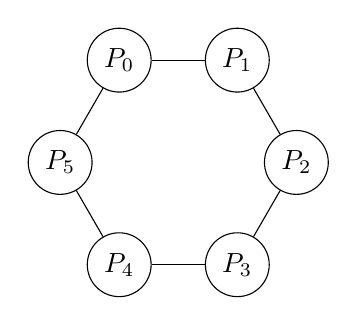
\begin{tikzpicture}[x=1.5cm,y=1.5cm]
  \tikzstyle{every node}=[draw,circle]
  \draw
  (0,0)      node (0) {$P_0$}
  ++(   0:1) node (1) {$P_1$}
  ++( -60:1) node (2) {$P_2$}
  ++(-120:1) node (3) {$P_3$}
  ++(-180:1) node (4) {$P_4$}
  ++(-240:1) node (5) {$P_5$}
  ;
  \draw (0) -- (1);
  \draw (1) -- (2);
  \draw (2) -- (3);
  \draw (3) -- (4);
  \draw (4) -- (5);
  \draw (5) -- (0);
\end{tikzpicture}
\end{frame}

\begin{frame}
\begin{itemize}
\item Each process $P_i$ holds a variable $x_i$ which ranges from $0$ to $n$ ($x_i\in\Nat_{n+1}$). 
\item Each $P_i$ can read and write $x_i$ and can read $x_{i-1}$ (where subtraction   is modulo $n$). 
\item $P_0$ is said to have a token when it sees $x_{n-1} = x_0$. Any other $P_i$ has a token when $x_{i-1} \neq x_i$. 
\item Invariant
 \begin{itemize}
 \item A state is legitimate when exactly one process has the token, and I is the invariant state: 
\[ 
      \begin{array}{rrcl} 
         P_0: & x_{5} = x_0 & \to & x_0 \defeq x_0 + 1 \mod (n+1) 
  \\ P_{i>0}: & x_{i-1} \neq x_i & \to & x_i \defeq x_{i-1} 
      \end{array} 
\] 
 \end{itemize}
\end{itemize}
\end{frame}

\begin{frame}[allowframebreaks]
\frametitle{References}
\bibliographystyle{abbrv}
\bibliography{bibliography.bib}
\end{frame}

\end{document}

